%        File: computation_notes.tex
%     Created: Mon Dec 20 02:00 PM 2010 C
% Last Change: Mon Dec 20 02:00 PM 2010 C
%
\documentclass[a4paper]{article}
\usepackage[utf8]{inputenc}
\usepackage{graphicx}

\newcommand{\Spa}[1]{\mathbf{\hat{#1}}}
\newcommand{\Nspa}[1]{\mathbf{\underline{#1}}}
\newcommand{\Vec}[1]{\mathbf{#1}}
\newcommand{\figref}[1]{\figurename~\ref{#1}}

\begin{document}

\section{Computation of the velocity of a point on a rigid body using spatial
algebra}

The ABA computes automatically the spatial velocity of body $i$ in the
reference frame of the body such that computation of joint velocities are
easier. Now we want to compute the (linear) velocity in base coordinates of a
point $\Vec{p}$ that is attached to body $i$ with body coordinates
${}^i\Vec{r}_p$, i.e. we want to compute ${}^0 \Vec{\dot{r}}_p = {}^0
\Vec{r}_p$.

First of all we compute the spatial velocities ${}^0\Spa{v}$ of all bodies in
base coordinates (which can be done during the first loop of the ABA):

\begin{equation}
	{}^0\Spa{v}_i = {}^0\Spa{v}_{\lambda(i)} + {}^{0}\Spa{X}_{i} \Spa{v}_{Ji}
\end{equation}

where $\Spa{v}_{Ji} = \Spa{S}_i \dot{q}_i $ which is the velocity that is
propagated by joint $i$ from body $\lambda(i)$ to body $i$ along joint axis
$\Spa{S}_i$ (see also RBDA p. 80).

This is now the velocity of the body $i$ in base coordinates. What is now left
todo is to transform this velocity into the velocity of the point $\Vec{p}$.
Before we can do that we have to compute the coordinates of $P$ in base
coordinates which can be done by:

\begin{equation}
	{}^0\Vec{r}_p = {}^0 \Vec{r}_i + {}^0\Vec{R}_i {}^i \Vec{r}_p
\end{equation}

for which ${}^0 \Vec{r}_i$ is the origin of the bodies in base coordinates and
${}^0 \Vec{R}_i$ the orientation of the base relative to the body.

Now we can compute the velocity of point $\Vec{r}_p$ with the following
formulation:
\begin{equation}
	{}^0\Spa{v}_p = \textit{xlt}({}^0\Vec{r}_p) {}^0\Spa{v}_i =
	\left[
	\begin{array}{cc}
		\Vec{1} & 0 \\
		-{}^0\Vec{r}_p \times & \Vec{1}
	\end{array}
	\right]
	{}^0\Spa{v}_i
\end{equation}

By doing so, the linear part of the spatial velocity ${}^0\Spa{v}_p$ has the
following entries:
\begin{equation}
	{}^0\Spa{v}_p = \left[
	\begin{array}{c}
		\Nspa{\omega} \\
		-{}^0\Nspa{r}_p \times \Nspa{\omega} + {}^0 \Nspa{\Vec{v}}_i
	\end{array}
	\right]
	=
	\left[
	\begin{array}{c}
		\Nspa{\omega} \\
		{}^0 \Nspa{\Vec{v}}_i + \Nspa{\omega} \times {}^0 \Nspa{r}_p
	\end{array}
	\right]
\end{equation}

For which the bottom line is the term for linear velocity in the standard 3D
notation.

\section{Computation of the acceleration of a point on a rigid body using
spatial algebra}

The acceleration of a point depends on three quantities: the position of the
point, velocity of the body and the acceleration of the body. We therefore
assume that we already computed the velocity as described in the previous
section.

To compute the acceleration of a point we have to compute the spatial
acceleration of a body in base coordinates. This can be expressed as:
\begin{equation}
	\Spa{a}_i = {}^0\Spa{a}_{\lambda(i)}
	+ {}^{0}\Spa{X}_{i} \Spa{a}_{Ji}
\end{equation}
for which $\Spa{a}_{Ji} = \Spa{S}_i \ddot{q}_i + \dot{\Spa{S}}_i \dot{q}_i$.
The last term can be written as: $\dot{\Spa{S}} = \Spa{v}_i \times \Spa{S}_i$.

\begin{figure}[h!]
	\begin{center}
		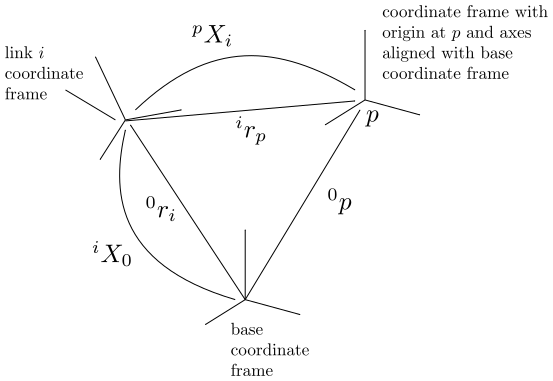
\includegraphics[width=0.9\textwidth]{acceleration_visualization}
	\end{center}
	\caption{Visualization of the acceleration of a point}
	\label{fig:acceleration_visualization}
\end{figure}

There are three coordinate systems involved in the computation of the
acceleration of point p which are shown in
\figref{fig:acceleration_visualization}. The \emph{base coordinate system}
which is the global reference frame, \emph{link $i$ coordinate system}
which is the coordinate system of body $i$, and the \emph{point coordinate
system} that is locate at the current position of $p$ and has the same
orientation as the base coordinate system.

First of all we build the transformation from the body coordinate system to
the point coordinate system:
\begin{equation}
	{^p}\Vec{X}_i =
	\left[
	\begin{array}{cc}
		{^0}\Vec{E}_i & \Vec{0} \\
		\Vec{0} & {^0}\Vec{E}_i
	\end{array}
	\right]
	\left[
	\begin{array}{cc}
		\Vec{1} & \Vec{0} \\
		-{^i}\Nspa{r}_p \times & \Vec{1}
	\end{array}
	\right].
\end{equation}
This can now be used to express the velocity and acceleration of the body at
the point p:
\begin{equation}
	{^p}\Spa{v}_i = {^p}\Vec{X}_i \Spa{v}_i
\end{equation}
\begin{equation}
	{^p}\Spa{a}_i = {^p}\Vec{X}_i \Spa{a}_i
\end{equation}

We now want to retrieve the \emph{classical acceleration}. It is expressed in a
coordinate frame that has a pure linear velocity of ${^0}\Nspa{\dot{p}}$.
\begin{equation}
	{^p}\Spa{a}'_i = {^p}\Spa{a}_i + 
	\left[
	\begin{array}{c}
		\Vec{0}\\
		{^0}\Nspa{\omega}_i \times {^0}\Nspa{\dot{p}}
	\end{array}
	\right]
\end{equation}

The linear part of this vector is then the acceleration of the point in base
coordinates.

\end{document}
